\documentclass[twocolumn,a4j]{jsarticle}
\setlength{\topmargin}{-20.4cm}
\setlength{\oddsidemargin}{-10.4mm}
\setlength{\evensidemargin}{-10.4mm}
\setlength{\textwidth}{18cm}
\setlength{\textheight}{26cm}

\usepackage[top=15truemm,bottom=25truemm,left=15truemm,right=15truemm]{geometry}
\usepackage[latin1]{inputenc}
\usepackage{amsmath}
\usepackage{amsfonts}
\usepackage{amssymb}
\usepackage[dvipdfmx]{graphicx}
\usepackage[dvipdfmx]{color}
\usepackage{listings}
\usepackage{listings,jvlisting}
\usepackage{geometry}
\usepackage{framed}
\usepackage{color}
\usepackage[dvipdfmx]{hyperref}
\usepackage{ascmac}
\usepackage{enumerate}
\usepackage{tabularx}
\usepackage{cancel}
\usepackage{scalefnt}

\renewcommand{\figurename}{Fig.}
\renewcommand{\tablename}{Table }

\lstset{
basicstyle={\ttfamily},
identifierstyle={\small},
commentstyle={\smallitshape},
keywordstyle={\small\bfseries},
ndkeywordstyle={\small},
stringstyle={\small\ttfamily},
frame={tb},
breaklines=true,
columns=[l]{fullflexible},
xrightmargin=0zw,
xleftmargin=3zw,
numberstyle={\scriptsize},
stepnumber=1,
numbersep=1zw,
lineskip=-0.5ex
}

\makeatletter
\def\@maketitle
{
\begin{center}
{\LARGE \@title \par}
\end{center}
\begin{flushright}
{\large 報告書 NO.07 - 4\quad\@date\quad\@author}
\end{flushright}
\par\vskip 1.5em
}
\makeatother

\setcounter{tocdepth}{3}

\author{来代 勝胤}
\title{令和3年度 11月 第4週 報告書}
\date{2021/11/25}

\begin{document}
\columnseprule=0.1mm

\maketitle
\section*{報告内容}
\begin{enumerate}[1.]
    \item 進捗状況
    \item 実験装置
    \item 実験結果
\end{enumerate}

\section{進捗状況}
今週は、実験に向けて簡易的な実験装置の組立を行った.
また、作用力実験における荷重の暫定的な換算結果から、
実験装置がどの程度変位するかの簡易的な算出を行った.
\section{実験装置の組立}
\section{実験装置のひずみ算出}
試験用のひずみセンサを選定するにあたって、
ひずみセンサの取付部が作用力によってどの程度変位するかを調べる必要がある.
ここで、簡単のため可能な限り切りのいい数字を使っておおよその変位量を算出した.
\begin{figure}[htbp]
    \footnotesize
    \begin{center}
        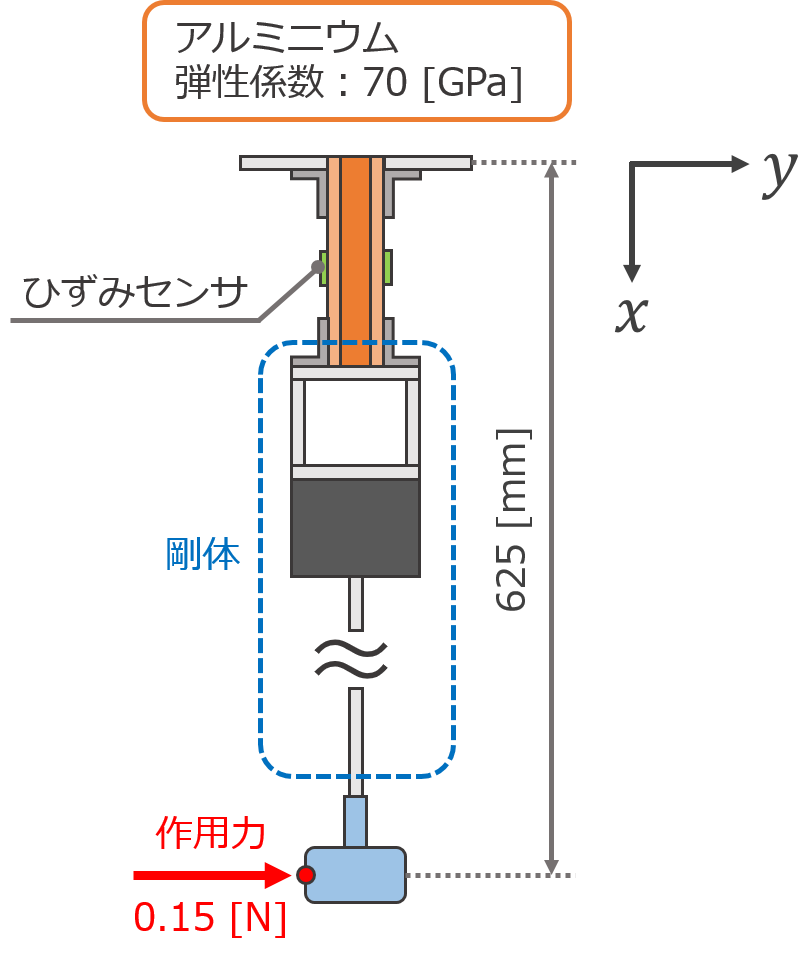
\includegraphics[width=70mm]{../images/moment.png}
        \caption{Cross-sectional shape of experimental device}
    \end{center}
\end{figure}
\subsection{算出結果}

\subsection{算出過程}
\begin{itembox}[l]{算出条件}
    \begin{itemize}
        \item [$\bullet$] アルミニウムの弾性係数  :$E = 70 \;\left[\mathrm{GPa}\right]$
        \item [$\bullet$] ひずみセンサと作用点の距離:$l = 625 \;\left[\mathrm{mm}\right]$
        \item [$\bullet$] 作用力          :$N = 0.15 \;\left[\mathrm{N}\right]$              
        \item [$\bullet$] 断面二次モーメント    :$I = 2701 \;\left[\mathrm{mm^4}\right]$              
        \item [$\bullet$] 取付部に加わるモーメント :$M$              
        \item [$\bullet$] たわみの曲率半径     :$R$              
        \item [$\bullet$] たわみ角         :$\theta$              
    \end{itemize}
\end{itembox}
\begin{itemize}
    \item [$\blacksquare$] 取付部に加わるモーメントの算出
    \begin{eqnarray*}
        M &=& N × \frac{l}{1000}\\
        &=& 0.15 × 0.625\\
        &=& 0.09375 \;\left[\mathrm{N \cdot m}\right]
    \end{eqnarray*}
    \item [$\blacksquare$] たわみの曲率半径の算出
    \begin{itembox}[l]{たわみの曲率半径}
        \begin{center}
            $\displaystyle \frac{1}{R} = \frac{M}{EI}$
        \end{center}
    \end{itembox}
    \begin{eqnarray*}
        R &=& \frac{EI}{M}\\
        &=& 70 × 2701 × \frac{100000}{9375}\\
        &\approx& 2016746.667 \left[\mathrm{mm}\right]
    \end{eqnarray*}
    \item [$\blacksquare$] たわみ角の算出
    \begin{itembox}[l]{たわみの微分方程式}
            \begin{center}
                $\displaystyle \frac{d^2w}{dx^2}=-\frac{M}{EI}$
                ※ 今回はひずみは正の値となる
            \end{center}
    \end{itembox}
    \begin{itembox}[l]{初期条件}
    \begin{itemize}
        \item [$\bullet$] $x=0$ のとき $w=0$,$\theta =0$
    \end{itemize}
    \end{itembox}
    \begin{eqnarray*}
        \frac{d^2w}{dx^2}&=&\frac{M}{EI}\\
        &=&\frac{0.09375}{70 × 2701}\\
        &=& 4.958 × 10^{-7} \left[\mathrm{1/mm}\right]\\ \\
        \frac{dw}{dx} &=& \frac{M}{EI} x + C_1\\ \\
        \frac{dw}{dx} &=& \frac{1}{2} \frac{M}{EI} x^2 + C_1x + C_2\\
    \end{eqnarray*}
\end{itemize}
\section{実験結果}
\end{document}